\documentclass[a4paper,12pt,oneside,pdflatex,italian,final,twocolumn]{article}

\usepackage[utf8]{inputenc}
\usepackage{parallel}
\usepackage{siunitx}
\usepackage{booktabs}
\usepackage{fancyhdr}
\usepackage{subcaption}
\usepackage{minted}
\usepackage{hyperref}
\usepackage{pdfpages}

\usepackage[export]{adjustbox}
\usepackage[margin=0.5in]{geometry}
\addtolength{\topmargin}{0in}

\usepackage{libertine}
\renewcommand*\familydefault{\sfdefault}  %% Only if the base font of the document is to be sans serif
\usepackage[T1]{fontenc}

\hypersetup{
	colorlinks=true, %set true if you want colored links
	linktoc=all,     %set to all if you want both sections and subsections linked
	linkcolor=blue,  %choose some color if you want links to stand out
	urlcolor=blue,   %url color
}

\definecolor{LightGray}{gray}{0.95}

\title{Halogen Flicker}
\author{Achmadi}
\date{July 2024}

\begin{document}
	\pagestyle{fancy}

	\lhead{Achmadi}
	\chead{\today}
	\rhead{Specification Document}

	\onecolumn
	\begin{figure}

	\end{figure}\begin{minipage}{0.47\textwidth}
		\centering

	\end{minipage}
	\hfill
	\begin{minipage}{0.47\textwidth}
		\raggedleft
		\Huge \textbf{Halogen Flicker v0}
	\end{minipage}

	\begin{figure}
		\begin{minipage}{0.47\textwidth}

			\section{Overview}
			\begin{itemize}
				\item Minimal and Flexible DC Power Control
				\item Based on Attiny13 and IRF540N
				\item Has mode options
				\item Simple to use
				\item Project Repository: \href{https://github.com/mekatronik-achmadi/short-jobs/tree/master/halogen-flicker}{Github}
			\end{itemize}

		\end{minipage}
		\hfill
		\begin{minipage}{0.47\textwidth}
			\centering
			\includegraphics[width=0.8\textwidth,right]{images/halodc_flicker_v0.png}
		\end{minipage}
	\end{figure}

	\raggedright
	
	\section{Firmware Draft}
	
	\begin{minted}[frame=lines,framesep=2mm,fontsize=\footnotesize,bgcolor=LightGray]{c}
#include <avr/io.h>
#include <util/delay.h>

#define FLICK_SLOW 1000
#define FLICK_FAST 200

#define FLICK_MODE_SLOW 0
#define FLICK_MODE_FAST 1

#define FLICK_FN _delay_ms
#define FLICK_MAX_CNT   6

static uint8_t flick_mode, flick_count;

int main(void)
{
	// CONTROL PIN
	DDRB |= 1<<3;
	PORTB &= ~(1<<3);
	
	flick_mode = FLICK_MODE_FAST;
	flick_count = 0;
	
	while (1) {
	  if(flick_mode==FLICK_MODE_FAST) FLICK_FN(FLICK_FAST);
	  else if(flick_mode==FLICK_MODE_SLOW) FLICK_FN(FLICK_SLOW);
		
	  PORTB ^= 1<<3;
	  flick_count++;
		
	  if(flick_count==FLICK_MAX_CNT){
	    if(flick_mode==FLICK_MODE_FAST) flick_mode=FLICK_MODE_SLOW;
		else if(flick_mode==FLICK_MODE_SLOW) flick_mode=FLICK_FAST;
		flick_count=0;
	  }
	}
	return 0;
}
	\end{minted}
	
	\section{Circuit Usage}

	\begin{figure}[h]
		\centering
		\includegraphics[width=\textwidth]{images/part.png}
		\caption{Circuit Usage}
	\end{figure}
	
	\section{Circuit Design}
	
	\includepdf[pages=-]{images/halodc_flicker_v0.pdf}
	
	\includepdf[pages=-]{images/halodc_flicker_v0__Assembly.pdf}

%	\section{Repository URLs}
%
%	\begin{itemize}
%		\item PCB Design: \url{https://github.com/deninur2427/ecu_pnm/tree/main/circuits/ecupnm_f051r8}
%
%		\item Firmware: \url{https://github.com/deninur2427/ecu_pnm/tree/main/firmware/}
%
%		\item Interface: \url{https://github.com/deninur2427/ecu_pnm/tree/main/interface/ecu_view/}
%
%		\item Overall Repository: \url{https://github.com/deninur2427/ecu_pnm/}
%	\end{itemize}
%
%	\section{Technical specification}
%	\centering
%	\begin{tabular}{lcr}
%		\toprule
%		Parts & Unit & Value \\
%		\midrule
%		Power voltage & $V$ & 12 \\
%		Main Chip & & STM32Fx LQFP64 \\
%		Storage & & Internal EEPROM \\
%		USB  Data Interface & & USB-Serial FT232RL \\
%		Engine Control Transistor & & IRF540N \\
%		TPS Input & & 12-bit ADC \\
%		PULSER Input & & Any pulsed signals \\
%		\bottomrule
%	\end{tabular}
%
%	\raggedright

%	\newpage
%	\section{Unit Preview}
%
%	\begin{figure}[h]
%		\centering
%		\begin{subfigure}{0.45\textwidth}
%			\includegraphics[width=\textwidth]{images/ecuparts.png}
%			\caption{Mockup}
%		\end{subfigure}
%		\begin{subfigure}{0.45\textwidth}
%			\includegraphics[width=\textwidth]{images/unit.png}
%			\caption{Actual}
%		\end{subfigure}
%	\end{figure}
%
%	\section{Electrical Wiring}
%
%	\begin{figure}[h]
%		\centering
%		\includegraphics[width=\textwidth]{images/wiring_lqfp64.png}
%		\caption{Electrical Wiring}
%	\end{figure}
%
%	\section{Schematic Design}
%
%	\includepdf[pages=-,angle=-90]{images/ecupnm_sch.pdf}
%
%	\newpage
%	\section{Firmware Summary}
%
%	In Summary:
%	\begin{itemize}
%		\item Library Framework: ChibiOS/RT
%
%		\item Running Mode: Real-Time Operating System
%
%		\item Compiler target: GCC ARM with Newlib for STM32 LQFP64 chip-series.
%	\end{itemize}
%
%	Some code snippet from \href[]{https://github.com/deninur2427/ecu_pnm/blob/main/firmware/ecu/main.c}{main.c}:
%
%	\begin{minted}[frame=lines,framesep=2mm,fontsize=\normalsize,bgcolor=LightGray]{c}
%int main(void) {
%	halInit();
%	chSysInit();
%
%	ecu_MEM_Init();
%	ecu_GPIO_Init();
%	ecu_SHELL_Init();
%	ecu_ICU_Init();
%	ecu_ADC_Init();
%	ecu_GPT_Init();
%
%	while (true) {
%		ecu_SHELL_Loop();
%		chThdSleepMilliseconds(500);
%	}
%}
%	\end{minted}
%
%	\section{Development Progress and Notes}
%
%	List of Development Notes:
%	\begin{itemize}
%		\item \href{https://github.com/deninur2427/ecu_pnm/blob/main/docs/notes/tes_31072023.md}{July 31\textsuperscript{st}, 2023}
%
%		\item \href{https://github.com/deninur2427/ecu_pnm/blob/main/docs/notes/tes_24082023.md}{August 24\textsuperscript{th}, 2023}
%	\end{itemize}

\end{document}
